% Options for packages loaded elsewhere
\PassOptionsToPackage{unicode}{hyperref}
\PassOptionsToPackage{hyphens}{url}
%
\documentclass[
  ignorenonframetext,
]{beamer}
\usepackage{pgfpages}
\setbeamertemplate{caption}[numbered]
\setbeamertemplate{caption label separator}{: }
\setbeamercolor{caption name}{fg=normal text.fg}
\beamertemplatenavigationsymbolsempty
% Prevent slide breaks in the middle of a paragraph
\widowpenalties 1 10000
\raggedbottom
\setbeamertemplate{part page}{
  \centering
  \begin{beamercolorbox}[sep=16pt,center]{part title}
    \usebeamerfont{part title}\insertpart\par
  \end{beamercolorbox}
}
\setbeamertemplate{section page}{
  \centering
  \begin{beamercolorbox}[sep=12pt,center]{part title}
    \usebeamerfont{section title}\insertsection\par
  \end{beamercolorbox}
}
\setbeamertemplate{subsection page}{
  \centering
  \begin{beamercolorbox}[sep=8pt,center]{part title}
    \usebeamerfont{subsection title}\insertsubsection\par
  \end{beamercolorbox}
}
\AtBeginPart{
  \frame{\partpage}
}
\AtBeginSection{
  \ifbibliography
  \else
    \frame{\sectionpage}
  \fi
}
\AtBeginSubsection{
  \frame{\subsectionpage}
}
\usepackage{lmodern}
\usepackage{amssymb,amsmath}
\usepackage{ifxetex,ifluatex}
\ifnum 0\ifxetex 1\fi\ifluatex 1\fi=0 % if pdftex
  \usepackage[T1]{fontenc}
  \usepackage[utf8]{inputenc}
  \usepackage{textcomp} % provide euro and other symbols
\else % if luatex or xetex
  \usepackage{unicode-math}
  \defaultfontfeatures{Scale=MatchLowercase}
  \defaultfontfeatures[\rmfamily]{Ligatures=TeX,Scale=1}
\fi
% Use upquote if available, for straight quotes in verbatim environments
\IfFileExists{upquote.sty}{\usepackage{upquote}}{}
\IfFileExists{microtype.sty}{% use microtype if available
  \usepackage[]{microtype}
  \UseMicrotypeSet[protrusion]{basicmath} % disable protrusion for tt fonts
}{}
\makeatletter
\@ifundefined{KOMAClassName}{% if non-KOMA class
  \IfFileExists{parskip.sty}{%
    \usepackage{parskip}
  }{% else
    \setlength{\parindent}{0pt}
    \setlength{\parskip}{6pt plus 2pt minus 1pt}}
}{% if KOMA class
  \KOMAoptions{parskip=half}}
\makeatother
\usepackage{xcolor}
\IfFileExists{xurl.sty}{\usepackage{xurl}}{} % add URL line breaks if available
\IfFileExists{bookmark.sty}{\usepackage{bookmark}}{\usepackage{hyperref}}
\hypersetup{
  pdftitle={UMCH Final Presentation},
  pdfauthor={STAT 245 Fall 2020 - Cora Boyoung Jung, Enoch Mwesigwa, Jordan Severn},
  hidelinks,
  pdfcreator={LaTeX via pandoc}}
\urlstyle{same} % disable monospaced font for URLs
\newif\ifbibliography
\setlength{\emergencystretch}{3em} % prevent overfull lines
\providecommand{\tightlist}{%
  \setlength{\itemsep}{0pt}\setlength{\parskip}{0pt}}
\setcounter{secnumdepth}{-\maxdimen} % remove section numbering

\title{UMCH Final Presentation}
\author{STAT 245 Fall 2020 - Cora Boyoung Jung, Enoch Mwesigwa, Jordan Severn}
\date{12/15/2020}

\begin{document}
\frame{\titlepage}

\begin{frame}

\end{frame}

\begin{frame}{UMCH}
\protect\hypertarget{umch}{}


\includegraphics[width=0.5\linewidth]{umch}

\end{frame}

\begin{frame}{Our Partner}
\protect\hypertarget{our-partner}{}

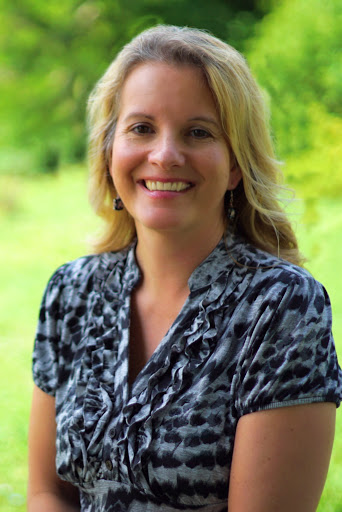
\includegraphics[width=0.2\linewidth]{michelle} *** Michelle A. Cossar\\
Director of Child Programs

\end{frame}

\begin{frame}{Goals}
\protect\hypertarget{goals}{}

\includegraphics[width=0.65\linewidth]{https://acamh.onlinelibrary.wiley.com/cms/asset/725a1afa-9bf2-485e-81ba-b6372bc62a30/jcpp12725-fig-0002-m}

\end{frame}

\begin{frame}{Data}
\protect\hypertarget{data}{}

\begin{itemize}
\item
  Response variable
\item
  Predictors
\item
  Model type
\item
  Interaction ?
\item
  Random effects ?
\item
  Model planning
\item
  Plots of the data
\item
  Coefficients, model summary information
\item
  Model assessment (condition checking)
\item
  Results of hypothesis testing or model selection
\item
  Model interpretation - what results mean
\item
  Prediction plots
\end{itemize}

\end{frame}

\begin{frame}{Experience}
\protect\hypertarget{experience}{}

What was the experience of working with your group/partner like? What
were strengths and weaknesses, joys or challenges? What would you
recommend/not to future groups; what lessons are learned? Can you
suggest structural changes to the class/projects that could help?

\end{frame}

\begin{frame}{Perspective}
\protect\hypertarget{perspective}{}

What would you love to do if you got to keep working on this dataset?
What mysteries remain, or what additional data would be enlightening? Do
you think your results will aid and inform your partner's work going
forward? How so?

Notes for perspective:

``If a larger dataset was available, it would be possible to get
estimates with less uncertainty and it would be possible to confirm or
refute whether there is an overall score difference by gender.\\
It would be interesting to have multiple datapoints for individual child
over time, so that we could be able to account for individual
differences and perhaps model how scores evolve over time. There are
many ways to improve this data analysis and one would be adding more
factors such as characteristics of the children, classrooms,
socio-economic status, or other demographics like race and ethnicity.
With more data, there are definitely more ways to go, more data to
explore, more predictions to make, and more conclusion to write.''

\end{frame}

\end{document}
